\section{Konstruktion des Aufbaus}

Für ein ressourcenschonendes Arbeiten ist es von großer Bedeutung neben den Methoden der Produktentwicklung auch diejenigen Materialien zu verwenden, die ohnehin schon vorrätig sind. In den entsprechenden Abschnitten wird noch näher drauf eingegangen. Zu bemerken sei aber noch, dass eine Verwendung der verfügbaren Materialien nicht immer die beste Option ist.

\subsection{Basisstativ}

In dem Labor \glqq Urban Mobility Lab\grqq\ liegt bereits das Fotostativ <Modell einfügen> bereit und kann verwendet werden. Herausfordernd kommt aber hinzu, dass sich ein 1/4\grqq\ Gewinde auf der Montageplatte befindet. Die folgenden Möglichkeiten zum Umgang mit dem Gewinde wurden diskutiert:

\begin{itemize}
	\item Nutenstein mit 1/4\grqq\ Innengewinde
	\item Adapterplatte zwischen Montageplatte und Trägerprofil
	\item Tausch der 1/4\grqq\ Schraube durch eine Schraube mit M4 Außengewinde
	\item Tausch des Stativs
\end{itemize}

Nach einer Anfrage bei item Industrietechnik GmbH nach Nutensteinen mit entsprechendem 1/4\grqq\ Innengewinde, war bekannt, dass sich derartige Produkte auf dem Markt nicht ohne Weiteres besorgen lassen.

Der Tausch des Stativs durch ein alternatives, ebenfalls zur Verfügung stehende, wurde ausgeschlossen, da die Dimensionen des Stativs eindeutig zu massiv sind und der Anforderung einer leichten Transportierbarkeit im Wege stehen.

Eine Adapterplatte aus einem Aluminium-Flachprofil wurde ausgeschlossen, da nach einer Untersuchung des Fotostativs sich herauskristallisiert hat, dass die eingebaute UNC Schraube einfach durch eine M4 Schraube getauscht werden kann.

\subsection{Mikrofongehäuse}

Dadurch, dass die zum Einsatz kommenden Mikrofone fertig auf einer Platine (\autoref{fig:Mikrofonplatine}) verbaut sind, aber damit nicht gegen Regenwasser geschützt sind, mussten im Entwicklungsprozess Gehäuse für die Mikrofone konstruiert und 3D-gedruckt werden. Nach sehr kurzer Diskussion war beschlossen, dass mittels CAD ein Gehäuse konstruiert und im vorhandenen 3D-Drucker gefertigt werden sollen (\autoref{fig:Mikrofongehäuse}).

\begin{figure}[h]
	\begin{center}
		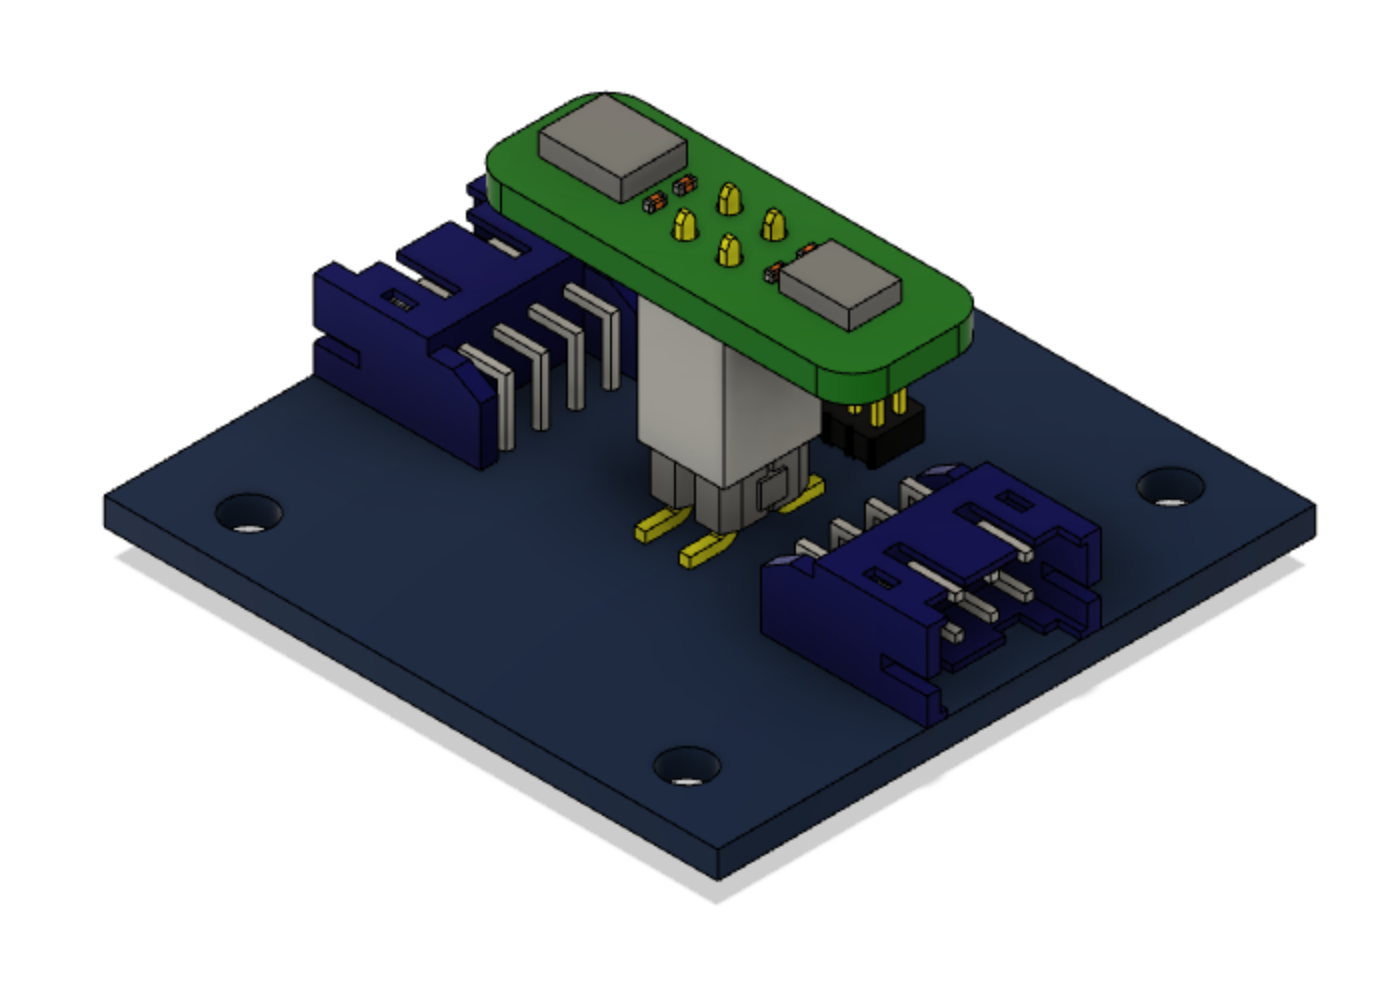
\includegraphics[scale=0.25]{Sections/Konstruktion_des_Aufbaus/Mikrofonplatine}
	\end{center}
	\caption{Mikrofonplatine}
	\label{fig:Mikrofonplatine}
\end{figure}

\newpage

\begin{figure}[h]
	\begin{center}
		\includegraphics[scale=0.25]{Sections/Konstruktion_des_Aufbaus/Mikrofongehäuse}
	\end{center}
	\caption{Mikrofongehäuse}
	\label{fig:Mikrofongehäuse}
\end{figure}

In der ersten Version dieser Gehäuse (\autoref{fig:Mikrofongehäuse_V_0.1}) soll die Mikrofonplatine über Stifte an Position gehalten und der Gehäusedeckel im Anschluss durch einen Längspressverband mit dem Gehäuseboden verbunden werden.

\begin{figure}[h]
	\begin{center}
		\includegraphics[scale=0.25]{Sections/Konstruktion_des_Aufbaus/Mikrofongehäuse_V_0.1}
	\end{center}
	\caption{Mikrofongehäuse V 0.1}
	\label{fig:Mikrofongehäuse_V_0.1}
\end{figure}


Nach dem Druck der sechs Gehäuse stellte sich heraus, dass:

\begin{enumerate}
	\item die gedruckten Stifte nicht zylindrisch und senkrecht sind
	\item der Durchmesser der Stifte mit den Durchmessern der Hüllen des Deckels nicht übereinstimmen
	\item viele druckbedingte Fäden an den Stiften beseitigt werden müssen
\end{enumerate}

An der gedruckten Geometrie lässt sich im Nachgang nicht mehr viel bearbeiten, lediglich die Hülsen im Gehäusedeckel können aufgebohrt werden. Die Erfahrung hat aber gezeigt, dass das verwendete Filament vor allem an den Kontaktflächen der einzelnen Layer zu porös ist und beim Aufbohren sehr schnell bricht. Alle Gehäuse wurden entsorgt.

Für die zweite Version der Gehäuse wurden die Stifte im Unterteil und die Hülsen im Deckel entfernt. Im Unterteil sind nun Sechskantaufnahmen für vier M2.5 Muttern und im Deckel Durchgangslöcher für entsprechend Lange Zylinderkopfschrauben. Durch Einpressen und Verkleben werden die Muttern nach dem Druck in die richtige Position gebracht, die Platine aufgelegt und das Gehäuse durch Anziehen der vier Schrauben geschlossen. Nach dem Druck eines neuen Prototyps wurde die Brauchbarkeit analysiert und das Gehäuse für die Massenproduktion freigegeben. Nachteilig ist, dass mit ausreichend großer Zugkraft die Gehäusedeckel trotz Verschraubung geöffnet werden können, zudem wirken die vier Schrauben etwas überdimensioniert. In einer zweiten Überarbeitung sollten diese beiden Punkte noch überarbeitet werden. (Abbildung einfügen)

\subsection{Unterbringung der Steuereinheit}

Für den Raspberry Pi 4, die Kamera und die Powerbank soll eine vorhandene wasserfeste Installationsbox verwendet werden (Modellbeschreibung einfügen). Das Hauptproblem war, die große Powerbank in der Box zu plazieren, daher wurde entschlossen eine neue Box zu bestellen (Modell einfügen). Für die sichere Positionierung aller Bauteile wird wieder auf die 3D-Druck-Technologie zurückgegriffen und ein Innenleben konstruiert.

Nach der ersten Konstruktion stellte sich heraus, dass die neu besorgte Installationsbox zu niedrig für das Innenleben ist, so dass bei einem Teamreview eine alternative Anordnung der Komponenten dazu führte, dass die besorgte Box verwendet werden kann. (Abbildungen einfügen)

\subsection{Positionierung der Baugruppen entlang eines Arrays}

Um die Mikrofone entlang einer Linie positionieren zu können, wurde ein \SI{1,1}{m} langes vorhandenes item-Profil eingesetzt, auf dem die Gehäuse der Mikrofone mit Nutensteinen in definiertem Abstand montiert werden können. Das Profil an sich wird, wie oben beschrieben, auch mittels eines Nutensteins auf dem Stativ befestigt. Für den Microcontroller wird eine wasserdichte Installationsbox auch mit Nutensteinen auf dem Profil montiert.

\newpage